\frame{
    \frametitle{Retention order pairs for preference learning}
    
\begin{block}{Notation}
\begin{itemize}
    \item Molecule $\mol_i$ from the molecular space $\molspace$
    \item $t_i\in\rettimespace$ its retention time
    \item $\sys_i\in\sysspace$ chromatographic system it has been measured with
\end{itemize}
\end{block}
\begin{block}{Pairwise molecule preference}
\begin{itemize}
    \item $\mol_i$ is preferred over $\mol_j$ when it \emph{elutes before} $\mol_j$, i.e. $t_i<t_j$
    \item Set of pairwise preferences of given LC-system $\sys$ is defined as:
\vspace{-0.15cm}
\begin{equation}
    \Pref(s)=\{(i,j)\,|\,\sys_i=\sys_j=\sys,t_i<t_j\}
\end{equation}
    \item Set of pairwise preferences from \emph{multiple} LC-systems:
\vspace{-0.15cm}
\begin{equation}
    \Pref=\bigcup_{\sys \in S} \Pref(\sys)
\end{equation}    
\end{itemize}
\end{block}
}

\frame{
    \frametitle{\ex{Retention order pairs for preference learning}}
    
    PUT EXAMPLE FIGURE HERE!
}

\frame{
    \frametitle{Ranking Support Vector Machine for molecular structures}
    
    We want to learn a pairwise retention order prediction function:
\vspace{-0.15cm} 
\begin{align}
    f(\mol_i = 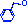
\includegraphics[scale=1.2]{images/mol_i.pdf},\mol_j = 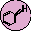
\includegraphics[scale=1.2]{images/mol_j.pdf} ) 
%         &= \sgn(\VEC{w}^T(\phi(\mol_j= 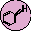
\includegraphics[scale=1.2]{images/mol_j.pdf})-\phi(\mol_i= 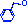
\includegraphics[scale=1.2]{images/mol_i.pdf})))\\
        &= \begin{cases}
            1  & \mol_i = 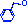
\includegraphics[scale=1.2]{images/mol_i.pdf} \text{ elutes before } \mol_j = 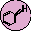
\includegraphics[scale=1.2]{images/mol_j.pdf}\\
            -1 & \text{otherwise}
        \end{cases}
\end{align}

\visible<2>{
\vspace{-0.75cm}
\begin{block}{Kernelized RankSVM prediction model}
\vspace{-0.15cm}
\begin{equation}
    f(\mol_i,\mol_j) = \sgn(\VEC{w}^T(\phi(\mol_j)-\phi(\mol_i)))
\end{equation}
\vspace{-0.15cm}
\begin{itemize}
    \item $\VEC{w}$ are the RankSVM model parameters
    \item Similarity between molecular structures is encoded by a \emph{kernel function} $\kmol:\molspace\times\molspace\rightarrow\mathcal{R}$.
    \item $\phi:\molspace\rightarrow\Fmol$ feature map associated with $\kmol$ embedding the molecular structures into a feature space.
\end{itemize}
\end{block}
}
}

\frame{
    \frametitle{Training the RankSVM for retention order prediction}
    
    We optimize $\VEC{w}$ considering the pairwise preferences $\Pref$ from different chromatographic systems:
\begin{align}
    \underset{\VEC{w},\VEC{\xi}}{\min} &\quad \frac{1}{2}\VEC{w}^T\VEC{w} + C\sum_{(i,j)\in  \Pref}\xi_{ij} \\
    s.t. &\quad\VEC{w}^T(\phi(\mol_j)-\phi(\mol_i))\geq 1-\xi_{ij}, \forall(i,j)\in  \Pref\label{prob:rankSVM-primal}\\
    &\quad \xi_{ij} \geq 0, \forall(i,j)\in \Pref,
\end{align}
    with $C>0$ being the regularization parameter.

\begin{block}{Learned model}
\begin{equation}
    \VEC{w}^T\phi(\mol_i)<\VEC{w}^T\phi(\mol_j),\,\text{if}\,(i,j)\in  \Pref 
\end{equation}
\end{block}
}
